\chapter{Konstrukcja modelu agentowego}\label{sec:theoreticalmodel}
Opis metod budowy modelu agentowego rynku podporządkujemy notacji zaczerpniętej z teorii systemów mikroekonomicznych \cite{smith82} - dziedziny podejmującej próbę usystematyzowania tworzenia syntetycznych rynków. Zgodnie z terminologią wprowadzoną przez tą dziedzinę model agentowy rynku $\mathcal{M}_{\mathbf{LOB}} = (\mathbf{E}, \mathbf{I})$ jest przykładem \textit{systemu mikroekonomicznego} złożonego z dwóch warstw:
\begin{itemize}
\item $\mathbf{E}$ - \textit{środowiska}: aktywów podlegających obrotowi oraz listy agentów z ustalonym uposażeniem, wiedzą oraz preferencjami,
\item  $\mathbf{I}$ - \textit{instytucji}: reguł "rzeczywistości", w której agenci funkcjonują - dopuszczalnej komunikacji między agentami oraz akcji, jakie mogą podjąć agenci.
\end{itemize}

Powyższy podział jest umotywowany przede wszystkim charakterem cech i informacji zawartych w obu składowych modelu. Elementy instytucji $I$ są publiczne i nie podlegają modyfikacji przez agentów, analogicznie do rzeczywistego prawa, regulacji giełdowych lub też fizycznych ograniczeń. Z kolei środowisko $E$ zawiera w sobie informacje natury prywatnej (zawartość portfela agenta, jego wierzenia i preferencje), które mogą ulegać zmianie pod wpływem decyzji agentów. 

Takie rozbicie elementów jest również zasadne w kontekście projektowania i implementacji modelu - reguły zawarte jako instytucja $I$ zwykle w dużej części można zaplanować jako bezpośrednie odwzorowanie rzeczywistych systemów lub ich uproszczenie, tymczasem sformułowanie w ścisły sposób często nieracjonalnych przekonań i decyzji agentów jest najbardziej nieoczywistym aspektem budowy modelu agentowego.  


\section{Odwzorowanie instytucji}
Instytucję $I$ możemy sformalizować jako zbiór praw (precyzyjniej: praw własności, ang. \textit{property rights}) wszystkich agentów uczestniczących w eksperymencie:
\begin{definition}\label{def:insitution}
\textbf{Instytucja} $I=\{I^1, ...,I^i, ...,I^N\}$ jest zbiorem praw przysługujących wszystkim agentom modelu. Zbiór praw $i.$ agenta składa się z: 
\begin{enumerate}[i.]
\item $M^i$ - możliwych wiadomości (akcji), którymi dysponuje agent, 
\item $h^i(m)$ - funkcji alokacji, rozstrzygającej zmianę stanu posiadania w wyniku wiadomości $m$, 
\item $c^i(m)$ - funkcji kosztu, rozstrzygającej koszty poniesione w skutku wiadomości $m$,
\item $g^i(t_0, t, T)$ - funkcji determinującej aktywność gracza w zależności od czasu, w szczególności: 
\begin{itemize}
\item $g^i(t_0,...,...)$: reguły startowe (ang.\textit{starting rules}),określające zachowanie agenta w momencie rozpoczęcia aukcji (otwarcia rynku),
\item $g^i(..., t, ...)$: reguły przejścia (ang.\textit{transition rules}),określające zachowanie agenta w trakcie trwania aukcji (sesji giełdowej),
\item $g^i(..., ..., T)$:reguły zatrzymania (ang.\textit{stopping rules}), określające zachowanie agenta w momencie zakończenia aukcji (zamknięcia rynku).
\end{itemize}  
\end{enumerate}
\end{definition}
\subsection{Komunikacja i język}\label{sec:language}
Kluczową składową instytucji jest \textit{język} $M=\bigcup_{i: e_i\in E} M^i$ - zbiór wszystkich możliwych wiadomości, które mogą wysłać agenci modelu. Zgodnie z metodologią budowy mikroekonomicznych modeli agentowych \cite{smith82} język modelu jest nietylko narzędziem komunikacji, przede wszystkim wyznacza możliwe akcje agentów. Każde publiczne działanie agenta modelu jest wynikiem jego interakcji z innym agentem (wymiany wiadomości), w przypadku zastosowania do rynku z arkuszem zleceń agent zdecydowany na kupno lub sprzedaż musi dokonać transakcji poprzez interakcję z agentem reprezentującym giełdę. 

Dla rynku opartego na arkuszu zleceń definiowanie języka $M$ dla modelu opiera się na bezpośrednim odwzorowaniu rzeczywistych protokołów wiadomości stosowanych przez giełdy, udostępnianych publicznie. W tej pracy korzystamy z języka opartego na protokołach OUCH \cite{ouch} i ITCH \cite{itch}. Oba protokoły zostały opracowane na potrzeby giełdy NASDAQ i stanowią współczesny standard wymiany wiadomości z giełdą. Język $M$ podzielimy na dwa podzbiory $M_O, M_D: M_O \cup M_D = M$, analogicznie do podziału zadań między protokołami OUCH i ITCH: 
\begin{itemize}
\item $M_O$ - wiadomości odpowiedzialne za obsługę zleceń i transakcji (analogicznie do OUCH),
\item $M_D$ - wiadomości odpowiedzialne za obsługę dostarczania danych rynkowych (przez mechanizmy zapytań i subskrypcji, analogicznie do ITCH).
\end{itemize}
Wewnątrz obu zbiorów wyróżnimy kolejne podzbiory zależne od nadawcy wiadomości: 
\begin{itemize}
\item $M_O = M^T_O \cup M^{EX}_O$: 
\begin{itemize}
\item $M^T_O$ - dyspozycje złożenia zlecenia giełdowego (wysyłane do giełdy przez kupujących lub sprzedających, ang. \textit{traders}), 
\item $M^{EX}_O$ - wiadomości informujące o stanie przetworzenia zlecenia, np. całkowitym lub częściowym zrealizowaniu (wysyłane wyłącznie przez agenta - giełdę); 
\end{itemize}
\item $M_D = M^T_D \cup M^{EX}_D$: 
\begin{itemize}
\item $M^T_D$ - zapytania o wartości konkretnych wskaźników rynkowych lub prośby o subskrypcję danych (wysyłane do giełdy przez zainteresowanych), \item$M^{EX}_D$ - wiadomości zwracające żądane dane oraz potwierdzenia złożenia lub anulowania subskrypcji (wysyłane przez giełdę). 
\end{itemize}
\end{itemize}
Zakładamy, że uczestnicy rynku operują na jednej giełdzie i mają równe możliwości handlu i komunikacji z giełdą (dysponują identycznymi zbiorami możliwych wiadomości $M^T = M^T_O \cup M^T_D$. 
\subsubsection{Wiadomości związane z obsługą zleceń}\label{sec:orderexecmsg}
Każdy agent modelu (poza agentem specjalnym $e_0$ reprezentującym giełdę) może wykonać następujące akcje na rynku z arkuszem zleceń:
\begin{itemize}
\item \textbf{złożenie zlecenia}: wysłanie zlecenia kupna lub sprzedaży wybranego typu (zlecenia z limitem ceny lub zlecenia po każdej cenie),
\item \textbf{anulowanie zlecenia}: wycofanie złożonej oferty kupna lub sprzedaży lub zredukowanie jej wielkości,
\item \textbf{modyfikacja zlecenia}: przez modyfikację rozumiemy zmianę parametrów zlecenia, która nie wpływa na jego pozycję w arkuszu zleceń (np. zwiększenie $\omega_x$ - wielkości oferty), 
\item \textbf{zastąpienie zlecenia}: obejmuje wszystkie możliwe modyfikacje zlecenia, wpływając przy tym na jego pozycję w arkuszu zleceń (np. zmianę ceny).
\end{itemize}
Wiadomości w języku $M$ modelu będące dyspozycjami powyższych czynności w większości tworzymy poprzez odtworzenie rzeczywistych komunikatów z protokołu OUCH (w tabeli \ref{tab:ordermsgtrader} przedstawione jest zestawienie wiadomości języka $M$ i ich odpowiedników w protokole). Wprowadzamy przy tym jedno istotne uproszczenie: ograniczamy możliwe typy składanych zleceń do dwóch bazowych (i zarazem najpowszechniej stosowanych) zleceń: zlecenia z limitem ceny (def. \ref{def:limitask}, \ref{def:limitbid}) oraz zlecenia po każdej cenie (def. \ref{marketorder}). Dla obu rozważanych typów zleceń zastępujemy rzeczywistą wspólną wiadomość \textit{Enter Order}, w której typ zlecenia jest określany przez bardzo szeroką parametryzację wiadomości, osobnymi wiadomościami dla dwóch typów zleceń rozważanych w modelu (\textit{LimitOrderMsg} i \textit{MarketOrderMsg}).
\begin{table}
\caption{Podstawowe wiadomości związane z obsługą zleceń wysyłane przez agentów-inwestorów} 
\label{tab:ordermsgtrader}

\begin{center}
\begin{tabular}{ |p{4.5cm}|p{4.5cm}|p{4.5cm}|}
\hline
\textbf{wiadomość} & \textbf{powiązana akcja agenta} &\textbf{odpowiednik w protokole OUCH} \\
\hline
\textit{LimitOrderMsg} & złożenie zlecenia z limitem ceny & \textit{Enter Order Message}[typ "O"] \\
\hline
\textit{MarketOrderMsg} & złożenie zlecenia typu \textit{market} (zlecenia po każdej cenie)& \textit{Enter Order} [typ "O"]\\
\hline
\textit{CancelOrderMsg} & anulowanie zlecenia & \textit{Cancel Order Request} [typ "X"]\\
\hline
\textit{PartialCancelOrderMsg} & anulowanie części zlecenia &\textit{Cancel Order Request} [typ "X"] \\
\hline
\textit{ModifyOrderMsg} & modyfikacja zlecenia & {Modify Order Request} [typ "M"]\\
\hline
\textit{ReplaceOrderMsg} & zastąpienie zlecenia nowym & \textit{Replace Order Message} [typ "U"]\\
\hline
\end{tabular} 
\end{center}
\end{table}
Agent reprezentujący giełdę w odpowiedzi na wiadomości agentów przeprowadza zlecone przez nich operacje: na życzenie nadawcy tworzy, modyfikuje i anuluje zlecenia. Dodatkowo po każdej transakcji z udziałem zlecenia aktualizuje jego stan, realizując całość kwoty zlecenia $\omega_x$ lub jego część. Każda z akcji zwieńczona jet wysłaniem komunikatu do agenta, który złożył dane zlecenie. Wiadomości powiązane z obsługą zleceń wysyłane przez agenta giełdy wraz z ich rzeczywistymi odpowiednikami opisane są w tabeli \ref{tab:ordermsgexchange}.
\begin{table}
\caption{Podstawowe wiadomości związane z obsługą zleceń wysyłane przez giełdę} 
\label{tab:ordermsgexchange}
\begin{center}
\begin{tabular}{ |p{4.5cm}|p{4.5cm}|p{4.5cm}|}
\hline
\textbf{wiadomość} & \textbf{powiązana akcja giełdy} &\textbf{odpowiednik w protokole OUCH} \\
\hline
\textit{OrderAcceptedMsg} & poprawne utworzenie zlecenia (spełnione zostały wymogi formalne) i umieszczenie w arkuszu zleceń & \textit{Order Accepted Message}[typ "A"] \\
\hline
\textit{OrderExecutedMsg} & zrealizowanie całej kwoty lub części zlecenia  & \textit{Order Executed Message}[typ "E"] \\
\hline
\textit{OrderCancelledMsg} & anulowanie zlecenia i usunięcie z arkusza zleceń & \textit{Order Canceled Message}[typ "C"] \\
\hline
\textit{OrderPartialCancelledMsg} & anulowanie części zlecenia & \textit{Order Canceled Message}[typ "C"] \\
\hline
\textit{OrderModifiedMsg} & dokonanie modyfikacji zlecenia & \textit{Order Modified Message}[typ "M"] \\
\hline
\textit{OrderReplacedMsg} & zastąpienie zlecenia nowym & \textit{Order Replaced Message}[typ "U"] \\
\hline

\end{tabular}
\end{center}

\end{table}

\subsubsection{Wiadomości związane z obserwacją rynku}

Oprócz wiadomości dających agentom możliwość kupna i sprzedaży na giełdzie oraz informujących o przebiegu tych czynności, język $M$ jest również wyposażony w wiadomości $M_D$ regulujące dostęp agentów do danych rynkowych: aktualnego stanu arkusza zleceń, statystyk zrealizowanych dotychczas transakcji (np. łącznej wartości transakcji, liczby transakcji, ceny ostatniej zrealizowanej transakcji). Zebranych danych agent może użyć jako wskaźnika przy podejmowaniu decyzji o kupnie lub sprzedaży albo do wyznaczenia ceny planowanego zlecenia. 

Zakładamy, że giełda może udostępnić agentowi dane z użyciem jednego z dwóch mechanizmów: odpowiedzi na zapytanie lub regularnego wysyłania danych w ramach zapisania się agenta do subskrypcji na dane. 

W naszym modelu zakładamy, że arkusz zleceń i jego charakterystyki (np. liczba aktywnych zleceń, ich ceny oraz sumaryczna wielkość) są publicznie dostępne dla wszystkich agentów poprzez zapytania i subskrypcje. Nie omówimy wszystkich danych udostępnianych przez giełdę, ograniczając się jedynie do przytoczenia kluczowych charakterystyk, które agenci modelu wykorzystują w procesie decyzyjnym:

\begin{itemize}
\item aktualnej ceny kupna $a(t)$ (def.\ref{def:askprice}),
\item aktualnej ceny sprzedaży $b(t)$ (def. \ref{def:bidprice}),
\item zrealizowanych dotychczas transakcji rynkowych (kupna i sprzedaży): $Y(t) = \{y = (p_y, \omega_y, t_y) : t_y \leq t\}$, w szczególności ostatniej zrealizowanej transakcji $y(t)$ ($y(t): t_{y'} = \max_{t_y: (p_y, \omega_y, t_y) \in Y(t)} t_y$).
\end{itemize}
Wymianę wiadomości odpowiedzialną za dostarczenie wyżej wymienionych danych przedstawia tabela \ref{tab:marketdata}.

\begin{table}
\caption{Wybrane wiadomości powiązane z dostarczaniem przez giełdę charakterystyk rynku} 
\label{tab:marketdata}
\begin{center}
\begin{tabular}{ |p{3.5cm}|p{4.5cm}|p{5cm}|}
\hline
\textbf{wiadomości agenta} & \textbf{wiadomości giełdy} &\textbf{dane} \\
\hline
\textit{QuerySpreadMsg} & \textit{QuerySpreadResponseMsg} & $t$ - czas wygenerowania wiadomości,\\
& & $a(t)$ - cena kupna,\\ 
& & $b(t)$ - cena sprzedaży,\\
& & $y(t) = (p_{y'}, \omega_{y'}, t_{y'})$ - ostatnia zrealizowana transakcja\\
\hline
\textit{MarketDataSubReqMsg}&\textit{MarketDataMsg} &$t$ - czas wygenerowania wiadomości  \\
& & $y(t) = (p_{y'}, \omega_{y'}, t_{y'})$ - ostatnia zrealizowana transakcja\\
\hline

\end{tabular}
\end{center}

\end{table}
% tu opisuję krótko pobierane dane i narzucam notację

% tu tabela z wiadomościami i danymi

\subsection{Reguły sprzedaży i kupna}\label{sec:marketrules}

Przebieg realizacji zleceń, podobnie do wiadomości, jest jednym z elementów, które możemy odwzorować bezpośrednio, zgodnie z mechanizmami opisanymi w sekcji \ref{sec:transactions}. W oparciu o ustalony sposób przetwarzania działań agentów i zbiór ich możliwych akcji regulowanych opisanym wyżej językiem $M$ możemy sprecyzować wymienione w definicji \ref{def:institution} $h^i(m)$ - funkcję alokacji oraz  $c^i(m)$ - funkcję kosztów. 

W bazowym modelu przyjmujemy założenie, że gracze, bez względu na typ wiadomości, nie ponoszą dodatkowych kosztów w związku z jej wysłaniem lub odebraniem. Zatem jedynymi wiadomościami, które będą zmieniały stan własności i majątek agentów będą potwierdzenia kupna lub sprzedaży wysyłane przez giełdę, czyli wiadomości typu \textit{OrderExecutedMsg}(opisane szerzej w sekcji \ref{sec:orderexecmsg}). Poniżej formalizujemy ich zawartość: 
\begin{definition}\label{def:ordexec}
\textbf{Potwierdzenie wykonania zlecenia} (\textit{OrderExecutedMsg}) $m_Y \in M$ to wiadomość wysyłana bezpośrednio po zrealizowaniu całości lub części kwoty zlecenia kupna (sprzedaży) przez agenta giełdy do nadawcy zlecenia. Zawiera następujące informacje: 
\begin{enumerate}[i.]
\item $t$ - czas wykonania, 
\item $\omega$ - liczba kupionych (sprzedanych) jednostek, 
\item $p$ - cena kupna (sprzedaży).
\end{enumerate}
\end{definition}
Na podstawie powyższego sformułowania możemy również sprecyzować format funkcji alokacji $h_i(m)$ i funkcji kosztów $c_i(m)$. Ze względu na to, że każdy z agentów (poza agentem-giełdą) ma równe możliwości handlu oraz dysponuje takim samym zestawem możliwych wiadomości $M^T = M^T_O \cup M^T_D$, działanie funkcji $h^i(m)$ i $c^i(m)$ będzie niezależne od agenta wyboru agenta $i$ ($\forall i \neq 0 : h^i(m) = h(m), c^i=c(m)$, gdzie $0$ - indeks agenta-giełdy). Wspólne funkcja alokacji $h(m)$ i funkcja kosztów $c(m)$ są postaci: 

$$ h(m) = 
 \left\{\begin{array}{lr}
        -\omega, & (m = m_Y) \wedge (\omega>0)\;\;\;\;\text{[sprzedaż]}\\
        \omega, & (m=m_Y) \wedge (\omega <0)\;\;\;\; \text{[kupno]}\\
        0, & m\neq m_Y \;\;\;\; \text{[inne wiadomości]}
        \end{array}
$$

$$ c(m) = 
 \left\{\begin{array}{lr}
        \omega \cdot p, & (m = m_Y) \wedge (\omega>0)\;\;\;\;\text{[sprzedaż]}\\
        -\omega \cdot p, & (m=m_Y) \wedge (\omega <0)\;\;\;\; \text{[kupno]}\\
        0, & m\neq m_Y \;\;\;\; \text{[inne wiadomości]}
        \end{array}
$$
gdzie $t$, $\omega$, $p$ zgodne z definicją $m_Y$ (def.\ref{def:ordexec}). 

Dla agenta-giełdy, który stanowi wyjątek, funkcje alokacji i kosztów nie będą zmieniały stanu własności giełdy: $g^0(m) = h^0(m) \equiv 0$. Przy założeniu braku opłat operacyjnych i prowizji giełda pełni jedynie rolę pośrednika między stronami. Innymi słowy, każdemu potwierdzeniu wykonania zlecenia kupna $x_B$ musi równolegle towarzyszyć potwierdzenie wykonania zlecenia sprzedaży $x_S$, które zostało przyporządkowane $x_B$ w drodze procedury dopasowywania zleceń (zgodnie z opisem w sekcji \ref{sec:transactions}).
\subsection{Aktywność agentów}\label{sec:agentactivity}
Ostatni element instytucji $I$ - funkcje aktywności agentów $g^i(t_0, t, T)$, jest najtrudniejszy do zaprojektowania. W przeciwieństwie do funkcji alokacji $h^i$ i funkcji kosztów $c^i$ wymaga indywidualnego sformułowania dla każdego z agentów. Funkcja $g^i$ określa zachowanie gracza (agenta) przy rozpoczęciu, w trakcie trwania oraz przy zakończeniu aukcji (sesji giełdowej), łącząc w sobie równocześnie dwa aspekty: strategię gracza oraz jego fizyczne ograniczenia w kwestii obserwacji rynku i uczestnictwa w aukcji. W pierwszej kolejności rozpatrzymy fizyczne ograniczenia agenta, do tematu strategii wracając w dalszej części rozdziału.

Przez fizyczne ograniczenia gracza (agenta) rozumiemy narzucenie momentów w czasie $\mathcal{T}^i = \{t_0, t^i_1, t^i_2, ..., T\}$ (tzw. obudzeń, ang.\textit{wakeups}), w których gracz może podjąć akcję. Wprowadzenie do modelu tego rodzaju ograniczeń wynika z założenia, że niektórzy agenci, naśladując zachowanie rzeczywistych inwestorów, nie są w stanie (lub nie mają potrzeby) obserwować rynku nieprzerwanie przez cały czas trwania sesji. Poniżej omówimy dwie metody wyznaczania zbioru obudzeń $\mathcal{T}^i$ agenta oparte na stylizowanych faktach nt. rynku z arkuszem zleceń, odzwierciedlające różne intencje odnośnie roli agentów.

\subsubsection{Momenty aktywności wyznaczone z rozkładu}
Jednym z podejść do wyznaczenia momentów aktywności agentów jest skorzystanie z empirycznych rozkładów sumarycznej wielkości złożonych zleceń (lub, alternatywnie, liczby zleceń) w zależności od czasu trwania sesji giełdowej. W tej technice zakładamy, że każdy z agentów wysyła tylko jedno zlecenie w ciągu trwania sesji giełdowej. W kontekście giełdy papierów wartościowych, na której się wzorujemy, to założenie nie stoi w sprzeczności z rzeczywistymi strategiami inwestorów - inwestycje w papiery wartościowe zwykle mają charakter długoterminowy.

Wyznaczając moment obudzenia $t^i$ agenta wykorzystujemy stylizowane fakty na temat aktywności agentów w zależności od czasu (Fakt \ref{fact:ushapeddist}), tzn. przyjmujemy, że suma wielkości zleceń $X(t) = \sum_{\{x=(p_x, \omega_x, t_x): t_x=t\}} \omega_x$ w czasie $t$ ma rozkład U-kształtny. Na potrzeby tej pracy przyjmiemy rozkład U-kwadratowy (\textit{U-quadratic}\ref{uquadratic}), tj:

$$ X(t) \sim f_{U_{t_0,T}}(t),$$

gdzie:

$$f_{U_{t_0,T, \alpha, \beta}}(t) = \alpha(t-\beta)^2, t\in[t_0,T], $$

parametry $\alpha$, $\beta$ zależne od przedziału $[t_0, T]$:
$$ \alpha = \frac{T+t_0}{2}, \beta=\frac{12}{(T-t_0)^3}.$$

W opracowaniach stylizowanych faktów \cite{abergel_lob} przeważnie nie określa się konkretnej funkcji gęstości rozkładu sumy wielkości zleceń w czasie $X(t)$, podkreślając jedynie U-kształtność - bimodalność ze zwiększonym prawdopodobieństwem dla wartości skrajnych (wykres ..), jako jego cechę charakterystyczną. Użycie rozkładu U-kwadratowego ma przede wszystkim uzasadnienie praktyczne. W celu wyznaczenia momentu obudzenia agenta $t^i$ generujemy próbę losową z założonego rozkładu $X(t)$. Używając rozkładu U-kwadratowego możemy to zrobić z użyciem funkcji odwrotnej dystrybuanty rozkładu $F_{U_{t0,T}$ (korzystając z własności $F^{-1}(U) \sim F, U\sim U(0,1)$ \cite{Devr86}), której wzór jesteśmy w stanie wyznaczyć analitycznie.
% tutaj dać wykres rozkładu q-kwadratowego - albo rozważyć danie go wcześniej

\subsubsection{Momenty aktywności jako proces Poissona}
% może tutaj trzeba nawiązać do jakiegoś dowodu?
%TODO: upewnić się odnośnie częstotliwośći parametrów
Alternatywnym podejściem do problemu wyznaczenia momentów aktywności agentów $\mathcal{T}^i$ jest interpretacja napływu zleceń na giełdę jako procesu Poissona. Takie rozwiązanie jest zgodne ze stylizowanymi faktami na temat rozkładu różnicy czasu między złożeniem dwóch zleceń. Zgodnie z faktem \ref{fact:interarrivals} czas między pojawieniem się na rynku dwóch kolejnych zleceń $\Delta_t$ ma rozkład wykładniczy $\mathrm{Exp(\lambda)}$, stąd proces zliczający liczbę zleceń w trakcie sesji giełdowej $N(t) = |\{x = (p_x, \omega_x, t_x): t_x \leq t\}|$ jest procesem Poissona z parametrem częstotliwości zdarzeń równym $\frac{1}{\lambda}$ \cite{lawler}. 

Parametr częstotliwości zleceń możemy wyznaczyć poprzez oszacowanie oczekiwanej liczby zleceń w jednostce czasu: $E[N(t)]= \frac{1}{\lambda}t$. Przy ustalonym parametrze $\lambda$ możemy wyznaczyć czasy złożenia kolejnych zleceń, generując wartości $\Delta_t$ z rozkładu wykładniczego. 

Opisaną powyżej procedurę indywidualizujemy dla każdego agenta, tzn. zakładamy że liczba obudzeń $i.$ gracza $|\mathcal{T}^i|$ w czasie (równoważnie liczba zleceń złożonych przez gracza) jest realizacją procesu Poissona $N^i(t)$ i jest zależna od parametru agenta $\lambda_i$. W ten sposób rozwiązujemy problem przyporządkowania kolejnych czasów aktywności różnym agentom, równocześnie wprowadzając możliwość zróżnicowania graczy na mniej i bardziej aktywnych. Warto zauważyć, że uzyskany w efekcie proces zliczający momenty złożenia zleceń dla wszystkich agentów $N'(t) = \sum_{i\in \{1,...,m\}} N^i(t)$ również jest procesem Poisssona: $N'(t)$ jest sumą $m$ niezależnych procesów Poissona  $N^1,..., N^m$ parametryzowanych odpowiednio parametrami $\lambda_1, ..., \lambda_m$, stąd $N'(t)$ jest procesem Poissona z parametrem $\lambda' = \sum_{i\in \{1,...,m\}}\lambda_i$ \cite{lawler} i zachowana jest zgodność ze stylizowanymi faktami na temat napływu zleceń na giełdę.
% cy tu wrzucić algorytm tego generowania?
\section{Agenci}
% przeczytać bibliometric bleble ble +
%przeczytać/przejrzeć get real +
% przeczytać/przejrzeć lob +
% rozdział o agentach 
% rozdział o abidesie 
% opis case study 
% opis konstrukcji informera 
% opis konstrukcji followera
% funkcja konfigruacyjna do symulacji 
% funkcje do analizy wyników symulacji 
% perfect rational,zero intelligence
Agentów $e^i \in E$ będziemy charakteryzować trzema podstawowymi atrybutami: 
\begin{enumerate}[i.]
\item $u^i$ - funkcją użyteczności, bazującą na indywidualnej wycenie instrumentu dokonanej przez agenta,
\item $\omega^i$ - ilością posiadanych jednostek instrumentu, 
\item $z^i$ - wielkością kapitału.
\end{enumerate}
Historycznie ukształtowały się dwa nurty \cite{lobbib} projektowania agentów ekonomicznych syntetycznych rynków: 
\begin{enumerate}[I.]
\item Agenci w pełni racjonalni (ang. \textit{Perfect-Rationality})
\item Agenci podejmujący losowe decyzje (ang. \textit{Zero Intelligence})
\end{enumerate}
Pierwsze podejście wywodzi się z teorii ekonomii. Kluczowym w nim jest założenie, że wszyscy agenci działają w pełni racjonalnie, podejmując decyzje w taki sposób by zmaksymalizować $u^i$. Celem badań jest zrozumienie złożonego działania rynku - wyznaczenie potencjalnych strategii graczy i uzasadnienie efektywności rzeczywistych rynków, tzn. wytłumaczenie, w jaki sposób możliwy jest handel przy spotkaniu się dwóch stron o sprzecznych interesach (kupujący chcą kupić możliwie najtaniej, podczas gdy sprzedający chcą sprzedać możliwie najdrożej).

Drugi istotny kierunek badań - agenci typu \textit{Zero Intelligence}, ma swoje korzenie w fizyce, a dokładniej w jej gałęzi wyspecjalizowanej w modelowaniu zjawisk ekonomicznych, ekonofizyce. Ekonofizycy kierują się inną motywacją niż ekonomiści - nadrzędnym celem rozwijanych przez nich modeli jest realistyczne odtworzenie napływu zleceń i stanu arkusza zleceń $\mathcal{L}(t)$ w czasie. Wychodzą przy tym od założenia, że indywidualne strategie uczestników rynku i ich optymalność mają marginalny wpływ na czas i rozkład wielkości przybywających zleceń \cite{godesunder}.

Modele agentowe rynku czerpią z dokonań obu grup, próbując zbudować model uniwersalny: równocześnie wiernie odtworzyć napływ zleceń i kształtowanie się ceny, i znaleźć uzasadnienie niektórych wzorców i tendencji występujących na rynku w racjonalnych zachowaniach agentów. Trudno przy tym jednoznacznie wskazać frakcję, która wywarła większy wpływ na współczesną formę modeli agentowych rynku \cite{lobbib}. Oprócz fizyków i ekonomistów, niejednokrotnie na kształt agentów wpływają również współtworzący modele praktycy, przekładający na projekty agentów swoje własne doświadczenia i obserwacje.
\begin{center}
\begin{figure}
\begin{center}
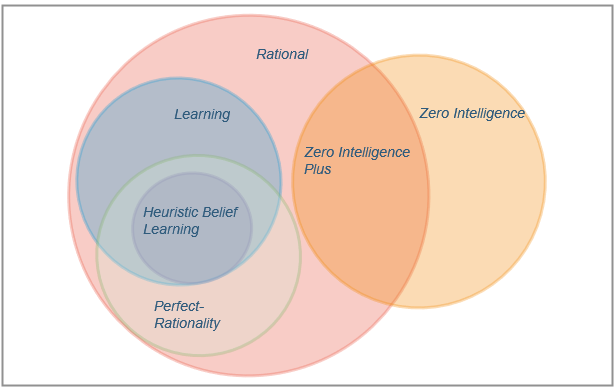
\includegraphics[scale=0.85]{agenci_venn.png}
\end{center}
\caption{Podstawowe klasy agentów na syntetycznych rynkach}\label{fig:agentsvenn}
\end{figure}
\end{center}
Finalnie modele agentowe często mają budowę będącą mieszanką koncepcji wywodzących się z rozwijanych wcześniej odrębnie wątków. Zbiór agentów w modelu ma charakter niejednorodny, zawiera różne typy agentów. Jest to uzasadnione istnieniem rzeczywistych grup graczy o odmiennych motywacjach (np. oczywistym podziałem jest podział na spekulantów i inwestorów długoterminowych). Dodatkowo zostało to również poparte analizą porównawczą, która wskazała, że modele ze zróżnicowanym zbiorem graczy znacząco lepiej odwzorowują stylizowane fakty nt. rynku niż modele oparte wyłącznie na agentach typu \textit{Zero Intelligence} \cite{getreal}. Spośród typów agentów występujących we współczesnych modelach agentowych możemy wyodrębnić kilka najbardziej istotnych klas (zobrazowanych również na rys. \ref{fig:agentsvenn}): 
\begin{itemize} 
\item agentów w pełni racjonalnych, których konstrukcja wywodzi się z teorii ekonomii lub jest bezpośrednim odwzorowaniem typowego działania wybranego uczestników rynku (\textit{Rational Agents}),
\item agentów składających zlecenia w sposób losowy, zdefiniowanych analogicznie do agentów modeli ekonofizycznych (\textit{Zero Intelligence Agent}),
\item agentów uczących się - zmieniających sposób działania na podstawie historii swoich dotychczasowych akcji (\textit{Learning Agents}), 
\item agentów aplikujących racjonalne reguły decyzyjne, ale częściowo zależnych od czynników losowych, np. wyznaczających cenę zlecenia zależnie od losowego czynnika(\textit{Zero Intelligence Plus Agents}).
\end{itemize} 
\subsection{Agenci typu \textit{Heuristic Belief Learning}}
Spośród agentów w pełni racjonalnych i uczących się szczególne znaczenie ma podklasa agentów typu HBL (\textit{Heuristic Belief Learning}) \cite{hblagent}. Agenci typu $HBL$ zostali wprowadzeni przez ekonomistów aspirujących do wyjaśnienia, w jaki sposób uczestnicy rynku z czasem uczą się wyznaczać cenę swoich ofert tak, aby możliwie szybko znaleźć kupca (sprzedawcę). Agent typu HBL wyznacza cenę planowanej oferty kupna i sprzedaży w oparciu o swoje oszacowanie szansy (przekonanie), że zlecenie wystawione po tej cenie jest najkorzystniejszym ruchem pod względem zysku i czasu realizacji. Formalizując, agent wyznacza cenę składanej oferty kupna lub sprzedaży na podstawie wzoru: 

$$p^*_i(t)= \left\{\begin{array}{lr}
        \mathrm{argmax}_p (p^i-p)f^i_t(p)& \text{dla kupna,}\\
        \mathrm{argmax}_p (p-p^i)f^i_t(p)& \text{dla sprzedaży,}\\
        \end{array}$$
gdzie:
\begin{itemize}
\item $p^i$ - indywidualna wycena $p^i$ handlowanego obiektu (instrumentu), może być zależna od czasu $t$ i liczby aktualnie posiadanych jednostek $\omega^i$, 
\item $f^i_t(p)$ - funkcja przekonania (ang.\textit{belief}) -  heurystyka prawdopodobieństwa, że zlecenie zostanie z sukcesem zrealizowane po cenie $p$, wyznaczana na podstawie historii dotychczasowych zleceń. 
\end{itemize}
Poważną wadą agentów typu HBL jest ich złożoność - ich konstrukcja wymaga stałego zapisywania i przechowywania wszystkich zleceń historycznych złożonych na giełdzie. Nawet jeśli ograniczymy okres zapisywanej historii, do np. $n$ ostatnich jednostek czasu, nadal jest to zadanie dosyć obciążające, szczególnie przy założeniu, że większość agentów (lub wszyscy, analogicznie do oryginalnego modelu \cite{hblagent}) niezależnie korzysta z tego mechanizmu wyznaczania ceny.
\subsection{Agenci typu \textit{Zero Intelligence Plus}}\label{sec:ziplus}
W tej pracy będziemy rozważać głównie agentów typu \textit{Zero Intelligence Plus} - agentów, których akcje mogą być, w różnym stopniu, losowe. Zakres pojęcia \textit{Zero Intelligence Plus} jest przy tym bardzo szeroki. Obejmuje minimalne modyfikacje agentów całkowicie losowych \textit{Zero Intelligence}, ale też agentów stosujących rozbudowane racjonalne strategie, z elementem losowości wprowadzonym jedynie na etapie wyznaczenia ceny, wielkości lub czasu wysłania zlecenia\cite{abides_explanation}.

W kontekście modeli rozważanych w tej pracy wyjątkowo ważne są dwa podtypy agentów \textit{Zero Intelligence Plus}\cite{lux}:
\begin{itemize}
\item agenci podejmujący decyzje w oparciu o obserwację danych rynkowych (ang. \textit{chartists} - "wykresiści"),
\item agenci podejmujący decyzję w oparciu o oszacowanie wartości instrumentu na podstawie wyceny indywidualnej oraz informacji "z zewnątrz" (ang. \textit{fundamentalists} - "fundamentaliści").
\end{itemize}
Powyższy podział jest odbiciem rzeczywistości - strategie graczy giełdowych możemy podzielić na bazujące głównie na wycenie instrumentu niezależnej od danych mikroekonomicznych (analiza fundamentalna) oraz na strategie polegające na wskaźnikach - funkcjach danych rynkowych mających identyfikować aktualne tendencje (analiza techniczna). 

Strategie "wykresistów" są, przy założeniu wiernego odwzorowania elementu instytucji $I$, możliwe do bezpośredniego przeniesienia na projekt agenta modelu. Decyzje podejmowane są na podstawie wskaźnika - funkcji danych rynkowych, które gracz może pozyskać za pomocą zapytania lub subskrypcji od agenta-giełdy $e^0$. Inaczej jest w przypadku drugiej grupy - "fundamentalistów", gdzie potrzebujemy do konstrukcji wprowadzić element subiektywnej wartości handlowanego obiektu dla agenta, z uwzględnieniem oszacowania na podstawie wiedzy publicznej oraz osobistych preferencji. W tym celu wprowadzamy do modelu dwa nowe obiekty: wartość fundamentalną instrumentu $r_t$ utożsamiającą wiedzę publiczną na temat wartości instrumentu oraz wektory wartości prywatnych agentów $\Theta = \{\theta^1, ..., \theta^m\}$ określające ich preferencje (przekonania o potencjalnym zaniżeniu lub zawyżeniu wartości). 
\subsubsection{Wartość fundamentalna}
Motywacją analizy fundamentalnej jest przekonanie, że cena rynkowa nie odzwierciedla dobrze rzeczywistej wartości instrumentu finansowego reprezentowanej przez $r_t$ - wartość fundamentalną. Zgodnie z założeniami, $r_t$ powinna utożsamiać całość aktualnej informacji publicznej na temat instrumentu, nie będąc przy tym podatną na spekulację powodującą fluktuacje ceny rynkowej. Teoretyczna wartość fundamentalna $r_t$ nie jest znana, stąd szacujemy jej wartość $\hat{r}_t$ korygując cenę rynkową w oparciu o zbiorczą informację z wielu źródeł.

Opisana powyżej logika przekłada się również na agentów realizujących strategie oparte na analizie fundamentalnej w ramach modelu: każdy z agentów tego typu ustala na swój użytek prywatną estymatę wartości fundamentalnej $\hat{r}^i_t$. Uściślenia wymaga jednak format informacji publicznej. Proces łączenia faktów z różnych źródeł jest pomijany: agenci za pośrednictwem dedykowanego obiektu - wyroczni $O$ obserwują wartość $r_t + \epsilon^i_t$, czyli wartość fundamentalną obarczoną błędem losowym i na jej podstawie aktualizują prywatne oszacowane $\hat{r}^i_t$.

W dotychczasowych modelach agentowych nie wyłoniła się spójna konwencja generowania danych udostępnianych agentom przez wyrocznię $O$. Część modeli używa w charakterze wyroczni danych historycznych, część definiuje $r_t$ jako proces stochastyczny. W tej pracy rozważamy jedynie drugie z podejść, przyjmując założenie że zawarta w modelu wyrocznia $O$ reprezentuje realizację parametryzowanego procesu stochastycznego. Szczegóły założonego procesu stochastycznego i estymacji $\hat{r}^i_t$ przez agentów opiszemy na przypadku modelu referencyjnego w kolejnym rozdziale.
% czy opisać orenstein -uhlenbeck już tutaj?
%Motywacją do wprowadzenia pojęcia wartości fundamentalnej do strategii inwestycyjnych jest przekonanie, że cena rynkowa nie odzwierciedla dobrze rzeczywistej wartości instrumentu finansowego - odbiega od sprawiedliwej ceny, stale zaniżając ją lub zawyżając. 
%znaleźć jakieś źródło z definicjami analizy technicznej i fundamentalnej 

% parę ogólnych zdań
% wkleić diagram Venna 
% przyjęcie notacji 
%ZI vs racjonalni, w tym HBL - przegląd 
\subsubsection{Preferencje}\label{sec:preferences}

Preferencje agentów wyrażamy przy pomocy atrybutu wartości prywatnych $\theta^i$. Wartości prywatne wywodzą się z teorii aukcji \cite{auction_theory}. 

Zgodnie z teorią aukcji wartość prywatna reprezentuje indywidualną dla agenta wycenę obiektu aukcji. Z wykorzystaniem pojęcia wartości prywatnych zostało wyprowadzonych kilka modeli przekonań i wiedzy licytujących graczy. W dziedzinie modeli agentowych wykorzystywany jest przede wszystkich podstawowy model - model niezależnych wartości prywatnych (ang. \textit{independent private values}, IPV). 
Model IPV definiuje wyceny obiektu poszczególnych graczy $(V_1,..., V_m)$ jako niezależne zmienne losowe o rozkładach odpowiednio $F_1, F_2, ..., F_m$. W konsekwencji niezależności zmiennych losowych, poszczególni gracze nie znają nawzajem swoich prywatnych wycen. 

Pierwotnie model niezależnych wartości prywatnych został sformułowany dla tradycyjnych jednostronnych aukcji pojedynczego obiektu. Przyjmujemy wówczas, że każdy gracz przystępuje do aukcji z prywatną wyceną $v_i$ wylosowaną odpowiednio z rozkładu $F_i$ i podejmuje decyzje o uczestnictwie w licytacji w oparciu o funkcję użyteczności $u^i$ następującej postaci:
$$u^i(p) = v_i - p, $$
gdzie $p$ jest aktualną ceną. 

Giełda reprezentuje bardziej złożony typ aukcji - aukcję ciągłą obustronną (ang. \textit{continous double auction}, CDA). Model modyfikujemy więc na potrzeby modelowania sesji giełdowej \cite{lobspoofing}, adresując przy tym dwa problemy: 
\begin{enumerate}
\item Możliwość kupna (sprzedaży) wielu jednostek instrumentu.
\item Możliwość zmiany wartości fundamentalnej instrumentu w trakcie trwania aukcji. 
\end{enumerate}
Pierwszy z problemów rozwiązujemy zastępując pojedynczą wartość wyceny $v_i$ wektorem wartości $v^i = (v^i_1, v^i_2, ...v^i_l)$ z rozkładu $F_i$, określającym wycenę każdej kolejnej dokupionej (sprzedanej) jednostki (przy założeniu możliwego kupna maksymalnie $l$ jednostek). Odpowiedzią na drugi problem jest rozbicie wyceny $v^i_j$ na dwa niezależne komponenty: 
$$v^i_j = r_t + \theta^i_j, $$
gdzie $r_t$ jest aktualną wartością fundamentalną handlowanego instrumentu, natomiast $\theta^i_j \in \theta^i$ wyraża preferencję zakupu $j$-tej jednostki. 
Scalając oba powyższe pomysły i dokładając możliwość handlu w dwie strony (kupna i sprzedaży równocześnie) wyposażamy $i$-tego gracza w następujący wektor preferencji $\theta^i$: 
$$\theta^i = (\theta^i_{-s}, \theta^i_{-j+1}, ...,\theta^i_{0}, ...,\theta^i_{l-1}, \theta^i_{l}),$$
gdzie $s$ - maksymalna liczba jednostek, które agent $i$ może sprzedać,$l$ - maksymalna liczba jednostek, które agent $i$ może kupić. Wartości $\theta^i_j\in \theta^i$ są z rozkładu $F'_i$. Zwykle przy stosowaniu w modelu agentowym przyjmujemy założenie $\theta^i_{j_1} \leq \theta^i_{j_2}$ dla $j_1 \leq j_2$, tzn. zakładamy że każda kolejna nabyta jednostka jest dla gracza mniej warta od poprzedniej. 

Dopuszczamy dużą elastyczność w interpretacji $v^i$ i $\theta^i$. Można użyć wartości prywatnych do zobrazowania nieracjonalnych sympatii, ale można też użyć jej do rozróżnienia różnego poziomu wiedzy specjalistycznej między graczami. W klasycznym sprawiedliwym modelu rynku, w którym zakładamy równy dostęp do informacji preferencje $\theta^i$ przyznajemy graczom w sposób losowy, z reguły przyjmując wspólny rozkład $\tilde{F}$ dla wszystkich graczy. Dla każdego gracza generujemy próbę losową rozmiaru wektora $\theta^i$, $|\theta^i| = s+k$, następnie sortujemy ją rosnąco, by zachować założenie o maleniu chęci kupna wraz ze zwiększaniem się liczby posiadanych jednostek.

